\documentclass{oblivoir}
\usepackage{amsmath,amssymb,amsthm,kotex,mdframed,paralist,kswrapfig}

\newcounter{num}
\newcommand{\prob}
{\bigskip\noindent\refstepcounter{num}\textbf{문제 \arabic{num})}\par}

\newcommand{\subprob}
{\bigskip\noindent\textbf{추가문제 \arabic{num}-1)}\par}

\newcommand{\subprobb}
{\bigskip\noindent\textbf{추가문제 \arabic{num}-2)}\par}

\newcommand{\ans}{{\raggedleft\textbf{답 : (\qquad\qquad\qquad\qquad\qquad\qquad)}
\par}\bigskip\bigskip}


\newcommand\ga{\text{(가)}}
\renewcommand\na{\text{(나)}}


%%%
\begin{document}
\Large

\title{승재 16 - 6학년 2학기 - 09}
\author{}
\date{\today}
\maketitle
%\tableofcontents

\newpage


%
\prob
다음 그림과 같이 A, B 두 개의 원기둥이 있습니다.
1m를 굴러가는데 A는 20바퀴 회전하였고 B는 15바퀴 회전했습니다.
A, B의 밑면의 반지름의 비를 구하세요.

\begin{figure}[h!]
\centering
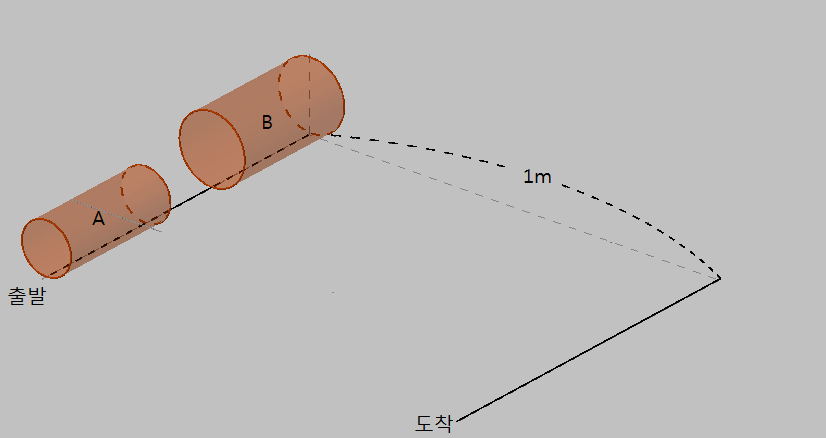
\includegraphics[width=0.7\textwidth]{01}
\end{figure}

\begin{mdframed}
\textbf{풀이 : }
\vspace{0.2\textheight}
\end{mdframed}
\ans

\newpage

%
\prob
다음 그림과 같이 A, B 두 개의 원기둥이 있습니다.
1m를 굴러가는데 A는 12바퀴 회전하였고 B는 16바퀴 회전했습니다.
A, B의 밑면의 넓이의 비를 구하세요.

\begin{figure}[h!]
\centering
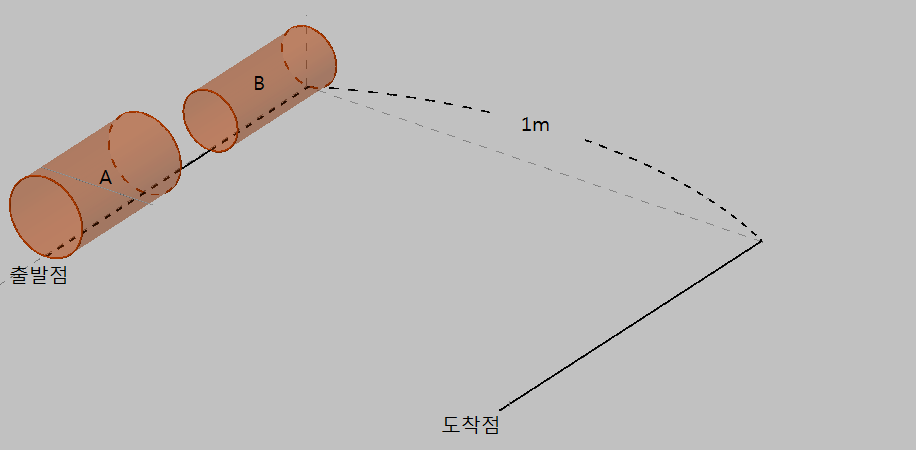
\includegraphics[width=0.7\textwidth]{02}
\end{figure}

\begin{mdframed}
\textbf{풀이 : }
\vspace{0.2\textheight}
\end{mdframed}
\ans

\newpage

%
\prob
다음 그림과 같이 밑면의 반지름의 길이와 높이가 같은 두 개의 원기둥 A, B가 있습니다.
두 원기둥에는 물감이 칠해져 있어서 굴러간 영역은 물감이 칠해집니다.
A가 15바퀴 회전하였고 B는 10바퀴 회전했을 때, A와 B의 바닥에 색칠된 영역의 넓이의 비를 구하세요.


\begin{figure}[h!]
\centering
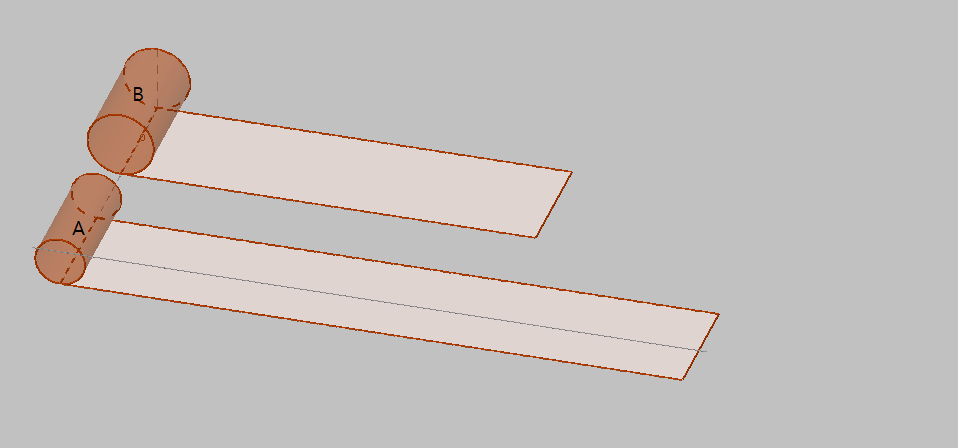
\includegraphics[width=0.7\textwidth]{03}
\end{figure}

\begin{mdframed}
\textbf{풀이 : }
\vspace{0.2\textheight}
\end{mdframed}
\ans
%
%\prob
%다음 그림과 같이 두 개의 원기둥 A, B가 있습니다.
%원기둥 A의 반지름의 길이는 원기둥 B의 반지름의 길이의 두 배이고 높이는 서로 같습니다.
%두 원기둥에는 물감이 칠해져 있어서 굴러간 영역은 물감이 칠해집니다.
%두 원기둥이 같은 횟수만큼 회전했을 때, A와 B의 바닥에 색칠된 영역의 넓이의 비를 구하세요.
%
%\ans
\newpage

%
\prob
선분 AB와 선분 BD의 길이의 비는 2:5이고 선분 AC와 선분 CD의 길이는 서로 같습니다.
\begin{figure}[h!]
\centering
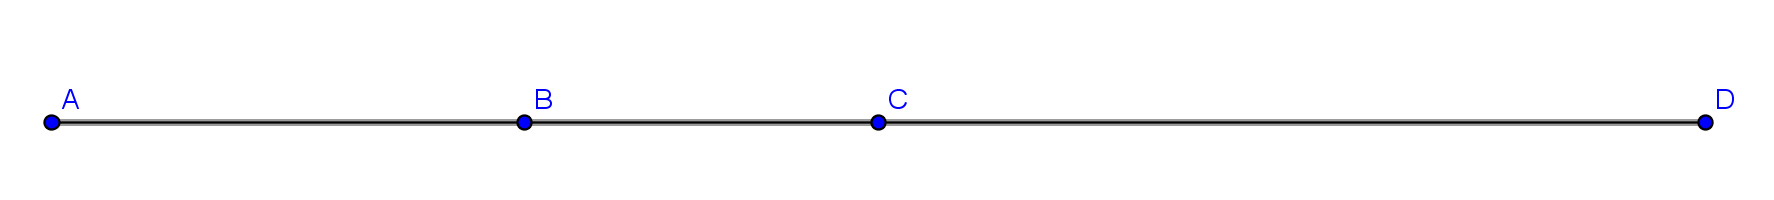
\includegraphics[width=0.9\textwidth]{04}
\end{figure}

이때, 선분 AB, 선분 BC, 선분 CD의 길이의 비를 구하세요.

\ans

%
\prob
선분 AB와 선분 BD의 길이의 비는 2:7이고 선분 AC와 선분 CD의 길이의 비는 5:1입니다.
\begin{figure}[h!]
\centering
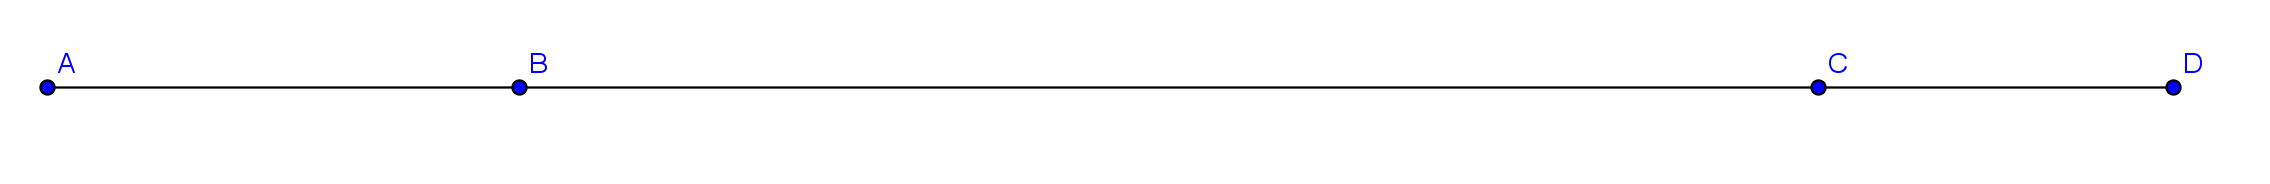
\includegraphics[width=0.9\textwidth]{05}
\end{figure}

이때, 선분 AB, 선분 BC, 선분 CD의 길이의 비를 구하세요.

\ans

\newpage

%
\prob
같은 크기의 옆면으로 만든 서로 다른 원기둥의 부피를 구하려고 합니다.
물음에 답하세오.
(원주율:3.1)
\begin{figure}[h!]
\centering
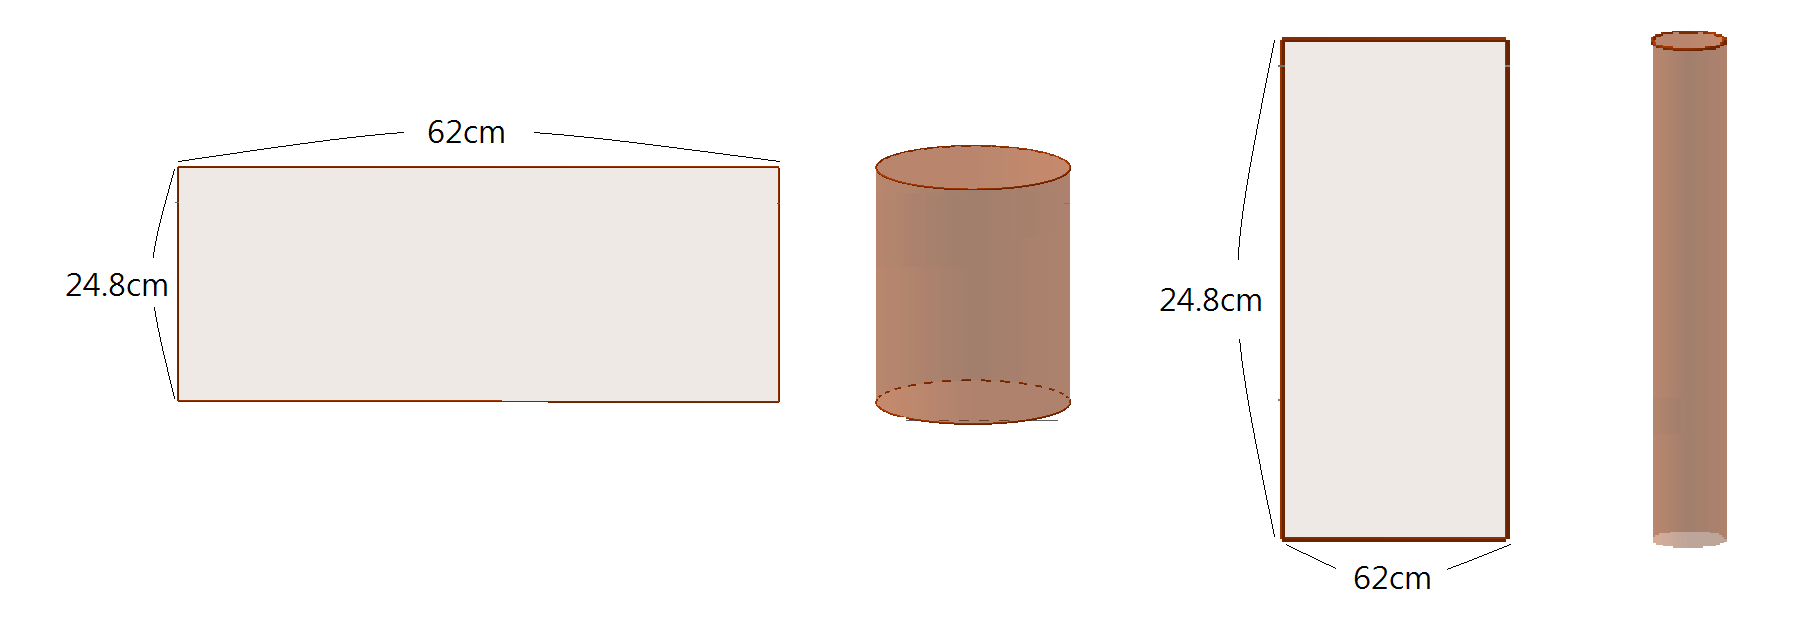
\includegraphics[width=0.9\textwidth]{08}
\end{figure}

(1) 직사각형 `가'를 옆면으로 하여 만든 원기둥의 부피는 몇 cm\(^3\) 입니까?

\ans

(2) 직사각형 `나'를 옆면으로 하여 만든 원기둥의 부피는 몇 cm\(^3\) 입니까?

\ans


\newpage
%
\prob
같은 크기의 옆면으로 만든 서로 다른 원기둥의 부피를 구하려고 합니다.
물음에 답하세오.
(원주율:3.1)
\begin{figure}[h!]
\centering
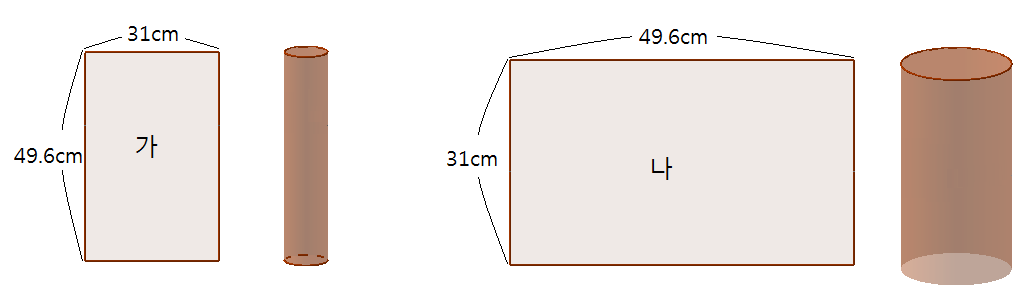
\includegraphics[width=0.9\textwidth]{09}
\end{figure}

(1) 직사각형 `가'를 옆면으로 하여 만든 원기둥의 부피는 몇 cm\(^3\) 입니까?

\ans

(2) 직사각형 `나'를 옆면으로 하여 만든 원기둥의 부피는 몇 cm\(^3\) 입니까?

\ans

\newpage

%
\prob
원기둥의 겉넓이가 785cm\(^2\)일 때 원기둥의 부피는 몇 cm\(^3\)입니까? (원주율 : 3.14)

\begin{figure}[h!]
\centering
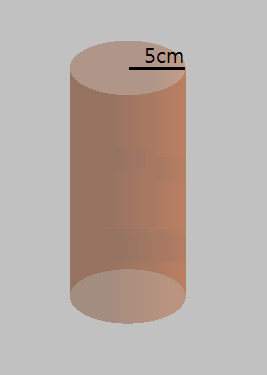
\includegraphics[width=0.3\textwidth]{14}
\end{figure}

\ans

%
\prob
원기둥의 겉넓이가 150.72cm\(^2\)일 때 원기둥의 부피는 몇 cm\(^3\)입니까? (원주율 : 3.14)

\begin{figure}[h!]
\centering
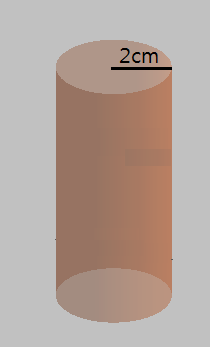
\includegraphics[width=0.3\textwidth]{15}
\end{figure}

\ans

\newpage
\prob
입체도형의 겉넓이는 몇 cm\(^2\)입니까?
(원주율:3.14)

\begin{figure}[h!]
\centering
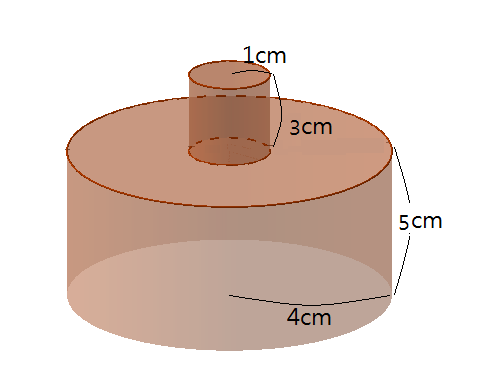
\includegraphics[width=0.9\textwidth]{10}
\end{figure}

\newpage
\prob
입체도형의 겉넓이는 몇 cm\(^2\)입니까?
(원주율:3.14)

\begin{figure}[h!]
\centering
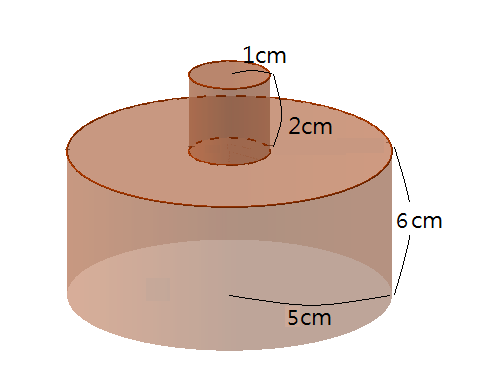
\includegraphics[width=0.9\textwidth]{16}
\end{figure}

\end{document}